\documentclass[11pt]{article}
\usepackage{csc766}

%%%%%%%%%%%%%%%%%%%% name/id
\rfoot{\small Brian Park | 200190057}


%%%%%%%%%%%%%%%%%%%% Course/HW info
\newcommand*{\instr}{Xipeng Shen}
\newcommand*{\term}{Spring 2023}
\newcommand*{\coursenum}{CSC 766}
\newcommand*{\coursename}{Code Optimization for Scalar and Parallel Programs}
\newcommand*{\hwnum}{2}

\rhead{\LARGE   \fontfamily{lmdh}\selectfont	HW \hwnum}

\lfoot{\small \coursenum, \term, HW \hwnum}

%%%%%%%%%%%%%%%%%%%%%%%%%%%%%% Document Start %%%%%%%%%%%%%%%%%
\begin{document}

%%%%%%%%%%%%%%%%%%%%%%%%%%%%%%%%%%%%%%%%%%%%%%%%%%%%%%%%%%%%%%%%%%%%%%%%%%%%%%%%%%%%%%%%
% Question 1
%%%%%%%%%%%%%%%%%%%%%%%%%%%%%%%%%%%%%%%%%%%%%%%%%%%%%%%%%%%%%%%%%%%%%%%%%%%%%%%%%%%%%%%%
\section{}

Convert the following loop to a form where the loop indexes are each incremented by 1:
\begin{verbatim}
for(i=50;i>=10;i=i-7) 
    X[i,i+1]=0;
\end{verbatim}

\begin{Answer}
	\begin{verbatim}
for(i=0;i<=5;i=i+1) 
    X[i*7+15,i*7+16]=0;
\end{verbatim}
\end{Answer}
\newpage
\section{}
\begin{enumerate}[a)]
	\item
	      \begin{verbatim}
for (i=1; i<30; i++)
    for (j=i+2; j<40-i; j++)
        X[i,j]=0;
\end{verbatim}

	\item
	      \begin{verbatim}
for (i=10; i<=1000;i++) 
    for (j=i; j<i+10; j++)
        X[i,j]=0;
\end{verbatim}

	\item
	      \begin{verbatim}
for (i=1; i<100; i++)
    for (j=0; j<100+i; j++)
        for (k=i+j; k<100-i-j; k++) 
            X[i,j,k]=0;
\end{verbatim}

\end{enumerate}
\begin{enumerate}
	\item Draw the iteration spaces for (a) and (b).
	      \begin{Answer}
		      \begin{figure}[H]
			      \centerline{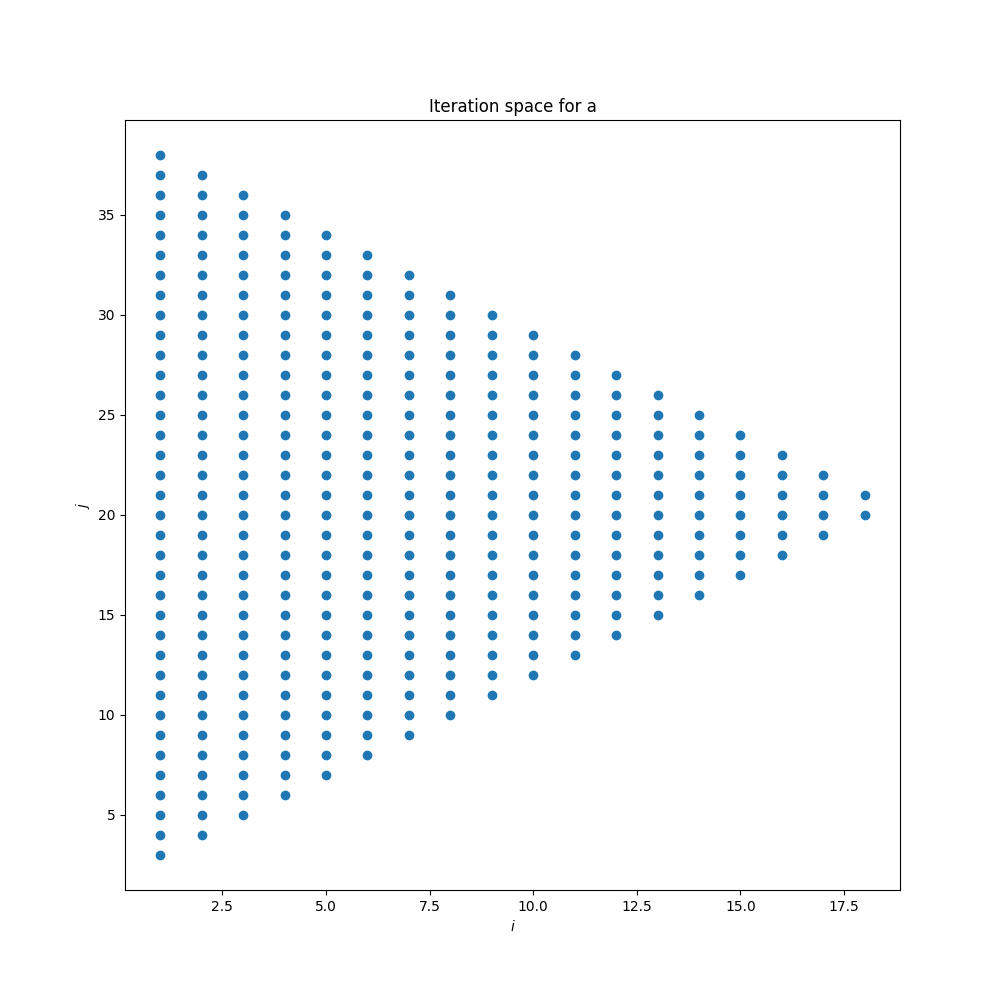
\includegraphics[width=6in]{figures/iteration_space_a.png}}
		      \end{figure}
		      \begin{figure}[H]
			      \centerline{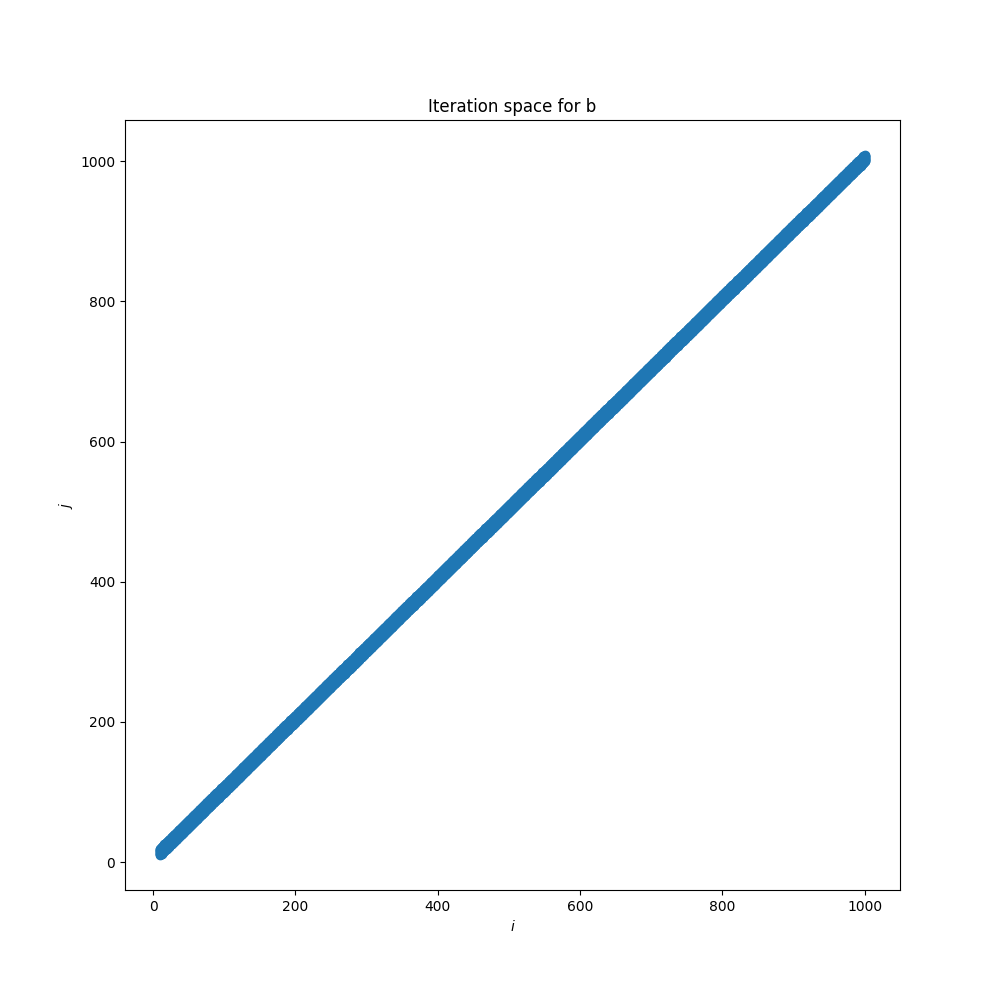
\includegraphics[width=6in]{figures/iteration_space_b.png}}
		      \end{figure}
	      \end{Answer}
	      \newpage
	\item Write the constraints in matrix form (i.e., give the values of the vectors $i$ and $b$ and the matrix $B$.)
	      \begin{Answer}
		      a.
		      $$
			      \begin{pmatrix}
				      1  & 0  \\
				      -1 & 0  \\
				      -1 & 1  \\
				      -1 & -1 \\
			      \end{pmatrix}
			      \begin{pmatrix}
				      i \\
				      j
			      \end{pmatrix}
			      +
			      \begin{pmatrix}
				      -1  \\
				      -29 \\
				      -2  \\
				      39
			      \end{pmatrix}
			      \ge
			      \begin{pmatrix}
				      0 \\
				      0 \\
				      0 \\
				      0
			      \end{pmatrix}
		      $$

		      b.
		      $$
			      \begin{pmatrix}
				      1  & 0  \\
				      -1 & 0  \\
				      -1 & 1  \\
				      1  & -1 \\
			      \end{pmatrix}
			      \begin{pmatrix}
				      i \\
				      j
			      \end{pmatrix}
			      +
			      \begin{pmatrix}
				      -10  \\
				      1000 \\
				      0    \\
				      9
			      \end{pmatrix}
			      \ge
			      \begin{pmatrix}
				      0 \\
				      0 \\
				      0 \\
				      0
			      \end{pmatrix}
		      $$

		      c.
		      $$
			      \begin{pmatrix}
				      1  & 0  & 0  \\
				      -1 & 0  & 0  \\
				      0  & 1  & 0  \\
				      1  & -1 & 0  \\
				      -1 & -1 & 1  \\
				      -1 & -1 & -1
			      \end{pmatrix}
			      \begin{pmatrix}
				      i \\
				      j \\
				      k
			      \end{pmatrix}
			      +
			      \begin{pmatrix}
				      -1 \\
				      99 \\
				      0  \\
				      99 \\
				      0  \\
				      99
			      \end{pmatrix}
			      \ge
			      \begin{pmatrix}
				      0 \\
				      0 \\
				      0 \\
				      0 \\
				      0 \\
				      0
			      \end{pmatrix}
		      $$
	      \end{Answer}
	      \newpage
	\item Use the Fourier-Motzkin elimination algorithm to eliminate $i$ from each of the sets of constraints obtained in the exercise (2).
	      \begin{Answer}
		      Transform constants using $m=j -i$, $j = m + i$, $i = j - m$. \\
		      a.
		      $$i \ge 1$$
		      $$i \le 29$$
		      $$j \ge i + 2$$
		      $$j \le 39 - i$$

		      Transform constants:
		      $$j - m \ge 1$$
		      $$j - m \le 29$$
		      $$j \ge j - m + 2$$
		      $$j \le 39 - j + m$$

		      $$j \ge m + 1$$
		      $$j \le m + 29$$
		      $$m \ge 2$$
		      $$m \ge 2j - 39$$
		      $$m \le 37$$

		      (from 1nd inequality $j - m \ge 1$

		      $$L_m = 2$$
		      $$U_m = 37$$
		      $$L_j = m + 1$$
		      $$U_j = m + 29$$

		      b.
		      $$i \ge 10$$
		      $$i \le 1000$$
		      $$j \ge i$$
		      $$j \le i + 9$$

		      Transform constants:
		      $$j - m \ge 10$$
		      $$j - m \le 1000$$
		      $$j \ge j - m$$
		      $$j \le j - m + 9$$

		      $$j \ge m + 10$$
		      $$j \le m + 1000$$
		      $$m \ge 0$$
		      $$m \le 9$$

		      $$L_m = 0$$
		      $$U_m = 9$$
		      $$L_j = m + 10$$
		      $$U_j = m + 1000$$

		      c.
		      $$i \ge 1$$
		      $$i \le 99$$
		      $$j \ge 0$$
		      $$j \le 99 + i$$
		      $$k \ge i + j$$
		      $$k \le 99 - i - j$$

		      $$j \ge m + 1$$
		      $$j \le m + 99$$
		      $$j \ge 0$$
		      $$m \le 99$$
		      $$k \ge 2j - m$$
		      $$k \le 99 - 2j + m$$

		      $$m \ge j - 99$$
		      $$m \le j - 1$$
		      $$j \ge 0$$
		      $$m \le 99$$
		      $$k \ge 2j - m$$
		      $$k \le 99 - 2j + m$$

		      $$j \ge 0$$
		      $$j \le m + 99$$
		      $$m \le - 1$$
		      $$m \le 99$$
		      $$k \ge 2j - m$$
		      $$k \le 99 - 2j + m$$


		      $$L_m = -1$$
		      $$U_m = 99$$
		      $$L_j = 0$$
		      $$U_j = m + 99$$
		      $$L_k = 2j - m$$
		      $$U_k = 99 - 2j + m$$
	      \end{Answer}
	      \newpage
	\item For each of the three loop nests, rewrite the code so the axis $i$ is replaced by the major diagonal, i.e., use loop index variable $m=j-i$. The new axis should correspond to the outermost loop.
	      \begin{Answer}
		      Transform constants using $m=j -i$, $j = m + i$, $i = j - m$. \\
		      a.
		      $$L_m = 2$$
		      $$U_m = 37$$
		      $$L_j = m + 1$$
		      $$U_j = m + 29$$
		      \begin{verbatim}
for (m=2; m<=37;m++)
    for (j=m+1; j<=m+29; j++)
        X[j-m,j]=0;
\end{verbatim}

		      b.
		      $$L_m = 0$$
		      $$U_m = 9$$
		      $$L_j = m + 10$$
		      $$U_j = m + 1000$$

		      \begin{verbatim}
for (m=0; m<=9;m++) 
    for (j=m+10; j<1000+m; j++)
        X[j-m,j]=0;
\end{verbatim}
		      c.
		      $$L_m = -1$$
		      $$U_m = 99$$
		      $$L_j = 0$$
		      $$U_j = m + 99$$
		      $$L_k = 2j - m$$
		      $$U_k = 99 - 2j + m$$

		      \begin{verbatim}
for (m=-1; m<99; m++)
    for (j=0; j<m+99; j++)
        for (k=2j - m; k<99 - 2j + m; k++) 
            X[j-m,j,k]=0;
\end{verbatim}
	      \end{Answer}
\end{enumerate}
\end{document}